\chapter{Syntax}\label{chap:syntax}

To describe the formal syntax of \gls{gamble} in order to parse the language it is necessary to write a \acrfull{cfg}.
Our grammar is written using \acrfull{ebnf}, and uses \acrfull{regex} for defining terminals such as numbers and names.

\section{Context-Free Grammar}
A \acrshort{cfg} is an areal of formal languages which are useful for specifying syntax. 
A \acrshort{cfg} generates a context-free language. 
A \acrshort{cfg} consists of one or several productions rules.
On the left side of a production rule is a nonterminal and on the right side are terminals and/or nonterminals, additionally there is a start symbol. % OG/ELLER HYPE!!!
An example of this written in \myref{lst:cfglst1}, here is a definition for multiplication and addition with parenthesis.
The grammar is structured such that the multiplication operator have a higher precedence than the addition operator.

\begin{lstlisting}[caption={An example of a \acrshort{cfg} written in \acrshort{ebnf}, with \acrshort{regex} for defining numbers. },frame=tlrb,label={lst:cfglst1},numbers=none]
expression = term | expression "+" term;
term       = factor | term "*" factor;
factor     = constant | "(" expression ")";
constant   = [0-9]+
\end{lstlisting}

It is possible to generate a parse tree for a string which follows the grammar. 
If there exists two or more trees for any given string then the grammar is ambiguous. 
Having an ambiguous grammar can be a problem when parsing.   
\todo{skriv om de transformationer man kan lave for at omgå ambiguous grammar}

There are two common strategy followed to generate a parse tree: the leftmost derivation and the rightmost derivation. 
A leftmost derivation always applies the rules in the grammar by always applying a production rule to the leftmost non-terminal. 
This is the strategy used in a top-down parser, also known as a LL parser.
A rightmost derivation is the reverse, and whats used in a bottom-up parser, also known as a LR parser. 

%For example take the string: ``1 + 3 * 4'', following PEMDAS this results in 13, if one were to simply calculate from left to right the result would be 16.
%A leftmost derivation would be:
%
%\begin{table}
%    \centering
%    \colorlet{shadecolor}{gray!40}
%    \rowcolors{1}{white}{shadecolor}
%    \begin{tabular}{|l|l|l|}
%    \hline
%    \textbf{Step} & \textbf{Sentential Form}           & \textbf{Production Number} \\ \hline
%    1    & \textit{expression}                &                   \\ \hline
%    2    & \textit{expression} ``+'' \textit{term}       & 1                 \\ \hline
%    3    & \textit{term} ``+'' \textit{term}             & 1                 \\ \hline
%    4    & \textit{factor} ``+'' \textit{term}          & 2                 \\ \hline
%    5    & \textit{constant} ``+'' \textit{term}         & 3                 \\ \hline
%    6    & 1 ``+'' \textit{term}                & 4                 \\ \hline
%    7    & 1 ``+'' \textit{term} ``*'' \textit{factor}     & 2                 \\ \hline
%    8    & 1 ``+'' \textit{constant} ``*'' \textit{factor} & 3                 \\ \hline
%    9    & 1 ``+'' 3 ``*'' \textit{constant}      & 3                 \\ \hline
%    10   & 1 ``+'' 3 ``*'' 4             & 4                 \\ \hline    
%    \end{tabular}
%    \caption{Existing GPU supporting languages}
%    \label{tbl:sota}
%\end{table}

\section{Classes of CFGs}
As mentioned there are two common strategies for parsing, leftmost and rightmost. 
A parser also has a lookahead which is the maximum numbers of tokens which are needed to determine what rule should be applied, this is denoted in a parenthesis, so i.e. LL(1) means leftmost derivation using a lookahead of 1 token. 
A lookahead of k means that there is a constant lookahead of a maximum of k tokens for the given parser. 
There also exists the LL(*) which can dynamically change the number of tokens needed to parse by recognising if they follow a \acrshort{regex}.
Combining this with the fact that any LL grammar is a special case of a LR grammar and the different cases of lookahead constructs a hierarchy. 
This hierarchy is shown in \myref{image:hierarchyofgrammars}, LL(*) not included.
In this figure is also contains the SLR which is more powerful than a LR(0) grammar, but less than a LR(1), and the LALR(1) which is more powerful than SLR and less than LR(1).
\begin{figure}[!ht]
\centering
 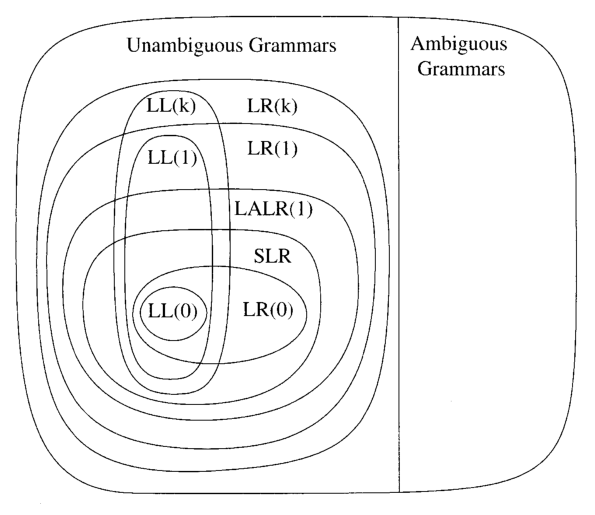
\includegraphics[width=0.5\textwidth]{figures/classesofgrammars.png} % trim=4.85cm 15cm 0.85cm 1cm
\caption{The hierarchy of \acrlong{cfg}. \citep{NvidiaCUDASeminar}}\label{image:hierarchyofgrammars}
\vspace{-15pt}
\end{figure}

